\chapter{Central Dogma of Molecular Biology}

The {\em central dogma of molecular biology} is a key idea that explains how genetic information is used in living organisms. Proposed by Francis Crick in 1958, it describes the flow of information from DNA to RNA to protein, which perform most of the vital functions in cells. This concept has been foundational to the field of molecular biology and continues to shape our understanding of genetics.

\begin{marginfigure}
    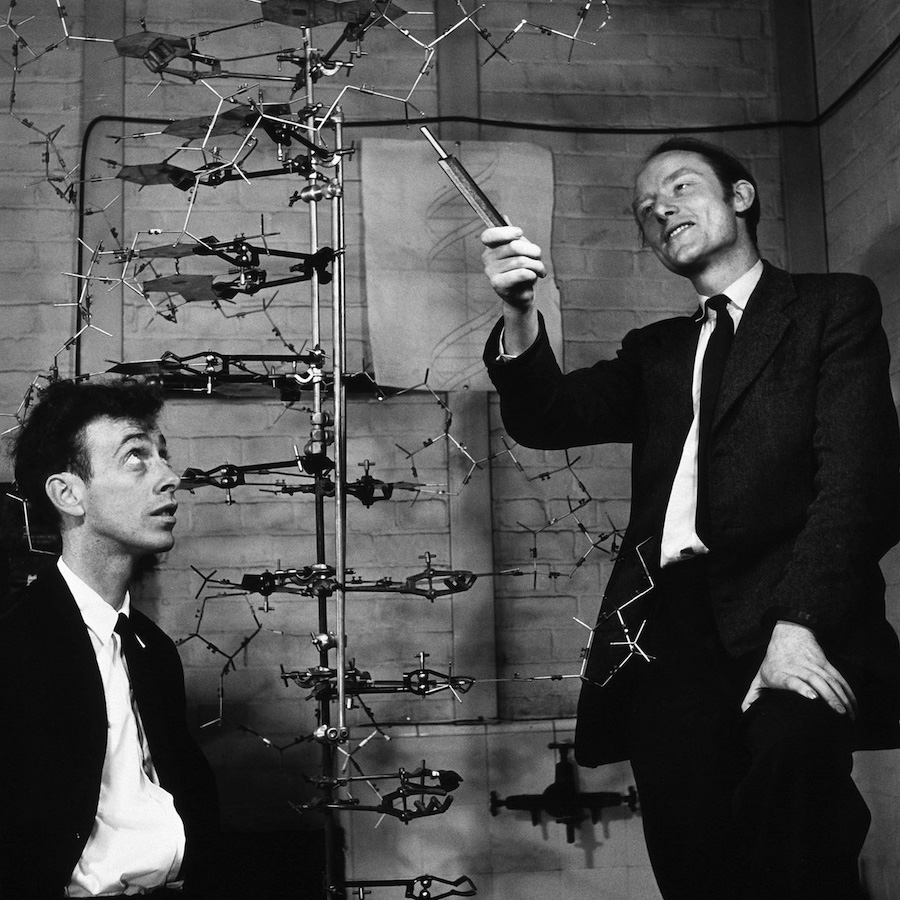
\includegraphics{figs/history/watson-crick-dna.jpeg}
    \caption[6pt]{Francis Crick and James Watson with their famous model of DNA.}
    \label{fig:watson-crick-dna}
\end{marginfigure}

Here are some of the major milestones, and some of the accompanying stories, in the development of the central dogma of molecular biology:

\medskip\noindent\textbf{1944:} Oswald Avery, Colin MacLeod, and Maclyn McCarty provided the first strong evidence that DNA is the genetic material. Studying pneumonia-causing bacteria, they found that traits such as virulence could only be transferred when DNA was present, while removing proteins or other molecules had no effect. At a time when most scientists assumed proteins carried genetic instructions because of their complexity, this experiment pointed instead to DNA as the true hereditary substance, a radical shift that set the stage for the discoveries that followed.

\medskip\noindent\textbf{1953:} The double-helix structure of DNA was uncovered by James Watson, Francis Crick, and Rosalind Franklin. Franklin’s X-ray diffraction work was critical to understanding the structure of DNA, although her contribution was underrecognized at the time. Without her clear images, the puzzle of DNA’s structure might have remained unsolved for much longer.

\begin{marginfigure}
    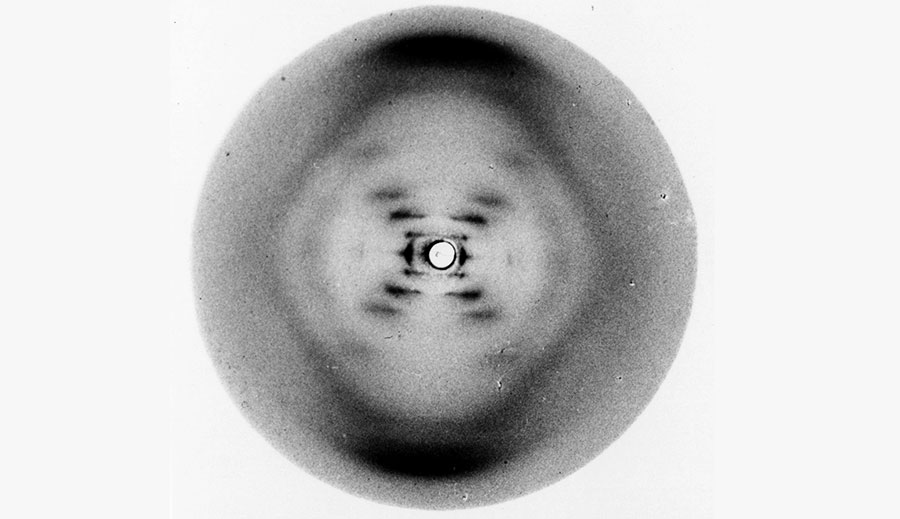
\includegraphics{figs/history/photograph-51.jpeg}
    \caption[6pt]{Photograph 51, the X-ray diffraction image of DNA taken by Rosalind Franklin.}
    \label{fig:photograph-51}
\end{marginfigure}

James Watson and Francis Crick's famous paper, titled "Molecular Structure of Nucleic Acids: A Structure for Deoxyribose Nucleic Acid," was published on April 25, 1953 in the journal Nature. This landmark paper was only about one page long, yet it had a profound impact on biology, as it described the double-helix structure of DNA for the first time.

Towards the end of Watson and Crick’s 1953 paper, they included a famous line:
\begin{quote}
    \textit{It has not escaped our notice that the specific pairing we have postulated immediately suggests a possible copying mechanism for the genetic material.}
\end{quote}
This sentence is understated yet profound. In a single line, Watson and Crick hint at one of the most important implications of their discovery: the double-helix structure of DNA naturally explains how genetic information can be copied during cell division. The specific pairing between the nucleotide bases (adenine with thymine, and guanine with cytosine) suggested a mechanism by which each strand of the DNA molecule could serve as a template for creating a new, complementary strand. This subtle but powerful insight laid the foundation for understanding DNA replication, a central process that ensures genetic continuity from one generation to the next. The modest tone belied its transformative impact on genetics and molecular biology.

Notice that the discovery of the structure of DNA was challenging and marked by missteps, even by the most influential scientists of the time. Linus Pauling, 
\marginnote{Pauling won the 1954 Nobel Prize in Chemistry for revealing the nature of the chemical bond, especially the covalent bond. His book \textit{The Nature of the Chemical Bond} became a classic and guided generations of chemists and biologists — including those who later solved the structure of DNA.}
one of the most renowned chemists of the era, proposed a triple-helix model for DNA in 1953, with the phosphate backbone in the center and the nucleotide bases on the outside. This model was fundamentally flawed due to charge repulsion between phosphate groups and its failure to account for base pairing. Pauling’s proposal, though influential, did not align with emerging data and was eventually replaced by the correct double-helix model proposed by Watson and Crick.

\medskip\noindent\textbf{1955:} Two major discoveries advanced the understanding of how genetic material is copied and used. Severo Ochoa identified an enzyme, polynucleotide phosphorylase, that could build RNA molecules in the lab, while Arthur Kornberg discovered DNA polymerase, the enzyme responsible for synthesizing new DNA strands inside cells. These breakthroughs showed that the copying of genetic information was a chemical process carried out by specific enzymes, providing the first direct tools to replicate and study DNA and RNA outside of living organisms.

\begin{marginfigure}
    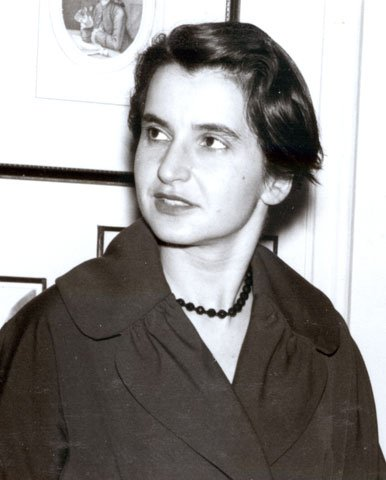
\includegraphics{figs/history/rosalind-franklin.jpeg}
    \caption[6pt]{Rosalind Franklin.}
    \label{fig:franklin}
\end{marginfigure}

\medskip\noindent\textbf{1958:} Francis Crick introduced the central dogma, explaining that information flows in one direction: from DNA to RNA to protein. Proteins carry out most cellular functions and are produced according to instructions stored in DNA.

\medskip\noindent\textbf{1961:} François Jacob and Jacques Monod discovered messenger RNA (mRNA), demonstrating that it carries instructions from DNA to the cell’s protein factories and acts as a temporary link in the process of turning genetic information into proteins.

\medskip\noindent\textbf{1966:} The cracking of the genetic code was a major scientific breakthrough. A group of scientists, including \textit{Marshall Nirenberg} and \textit{Har Gobind Khorana}, worked tirelessly to decipher how RNA sequences are translated into amino acids, the building blocks of proteins. At the same time, the \textit{RNA Tie Club}—an informal but competitive group of 20 scientists founded by George Gamow, each member representing one of the 20 amino acids—added a mix of humor and camaraderie to the effort. They even wore black silk ties emblazoned with the symbol for RNA.

One anecdote is that they created their own membership pins and issued bold declarations such as ``each amino acid will be solved by a club member!'' However, the race to crack the code was so competitive that, in the end, the discoveries were made by a few scientists outside the club. Still, the members’ friendly competition and idea-sharing helped push the field forward.

\bigskip\noindent\textbf{1970:} Howard Temin and David Baltimore discovered reverse transcriptase, an enzyme that allows RNA to be copied back into DNA. This discovery challenged the assumption that genetic information flows only from DNA to RNA and provided crucial insights into how retroviruses like HIV function.

\medskip\noindent\textbf{1977:} Phillip Sharp and Richard Roberts independently discovered that genes in higher organisms are not continuous but interrupted by non-coding regions, which they called introns. They showed that these introns are removed from the RNA transcript in a process known as splicing, leaving only the coding segments to be translated into protein. This finding overturned the simple view of genes as uninterrupted stretches of DNA and revealed an additional layer of complexity in how genetic information is processed.

\medskip\noindent\textbf{1980s:} The decade saw powerful new techniques that transformed molecular biology. In 1983, Kary Mullis developed the polymerase chain reaction (PCR), allowing scientists to rapidly amplify DNA sequences in the lab. Soon after, Leroy Hood’s team created the first automated DNA sequencing machines, opening the door to large-scale genomic projects. Together, these tools made it possible to copy, read, and analyze genetic material with unprecedented speed and accuracy.

\medskip\noindent\textbf{2000s:} The completion of the Human Genome Project in 2003 ushered in the genomics era. This international effort set out to determine the entire sequence of human DNA and identify all of its genes, producing a nearly complete genetic ``blueprint'' for our species. With this map, the central dogma expanded into a framework for studying how DNA, RNA, and proteins interact across the whole genome, fueling new fields such as personalized medicine, comparative genomics, and systems biology.

\bigskip\noindent
For computer scientists, the central dogma provides a blueprint for how biological data is organized. DNA is the database, RNA acts as a dynamic intermediary, and proteins are the functional executors. In bioinformatics, understanding these relationships is key to analyzing genetic sequences, predicting protein structures, and investigating the effects of mutations.